\documentclass[8pt,aspectratio=169]{beamer}
\usetheme{Madrid}
\usepackage{graphicx}
\usepackage{booktabs}
\usepackage{adjustbox}
\usepackage{multicol}
\usepackage{amsmath}
\usepackage{amssymb}
\usepackage{tikz}
\usetikzlibrary{arrows.meta,positioning,shapes.callouts,shapes.geometric,decorations.pathreplacing}
\usepackage{hyperref}
\usepackage{algorithm}
\usepackage{algorithmic}

% Color definitions
\definecolor{mlblue}{RGB}{0,102,204}
\definecolor{mlpurple}{RGB}{51,51,178}
\definecolor{mllavender}{RGB}{173,173,224}
\definecolor{mllavender2}{RGB}{193,193,232}
\definecolor{mllavender3}{RGB}{204,204,235}
\definecolor{mllavender4}{RGB}{214,214,239}
\definecolor{mlorange}{RGB}{255, 127, 14}
\definecolor{mlgreen}{RGB}{44, 160, 44}
\definecolor{mlred}{RGB}{214, 39, 40}
\definecolor{mlgray}{RGB}{127, 127, 127}

% Additional colors for template compatibility
\definecolor{lightgray}{RGB}{240, 240, 240}
\definecolor{midgray}{RGB}{180, 180, 180}

% Backward compatibility: uppercase color names
\colorlet{MLPurple}{mlpurple}
\colorlet{MLBlue}{mlblue}
\colorlet{MLOrange}{mlorange}
\colorlet{MLGreen}{mlgreen}
\colorlet{MLRed}{mlred}
\colorlet{MLLavender}{mllavender}
\colorlet{MLGray}{mlgray}

% Apply custom colors to Madrid theme
\setbeamercolor{palette primary}{bg=mllavender3,fg=mlpurple}
\setbeamercolor{palette secondary}{bg=mllavender2,fg=mlpurple}
\setbeamercolor{palette tertiary}{bg=mllavender,fg=white}
\setbeamercolor{palette quaternary}{bg=mlpurple,fg=white}

\setbeamercolor{structure}{fg=mlpurple}
\setbeamercolor{section in toc}{fg=mlpurple}
\setbeamercolor{subsection in toc}{fg=mlblue}
\setbeamercolor{title}{fg=mlpurple}
\setbeamercolor{frametitle}{fg=mlpurple,bg=mllavender3}
\setbeamercolor{block title}{bg=mllavender2,fg=mlpurple}
\setbeamercolor{block body}{bg=mllavender4,fg=black}

% Remove navigation symbols
\setbeamertemplate{navigation symbols}{}

% Clean itemize/enumerate
\setbeamertemplate{itemize items}[circle]
\setbeamertemplate{enumerate items}[default]

% Reduce margins for more content space
\setbeamersize{text margin left=5mm,text margin right=5mm}

% Custom course footer
\setbeamertemplate{footline}{
  \leavevmode%
  \hbox{%
    \begin{beamercolorbox}[wd=.333333\paperwidth,ht=2.25ex,dp=1ex,center]{author in head/foot}%
      \usebeamerfont{author in head/foot}Methods and Algorithms
    \end{beamercolorbox}%
    \begin{beamercolorbox}[wd=.333333\paperwidth,ht=2.25ex,dp=1ex,center]{title in head/foot}%
      \usebeamerfont{title in head/foot}MSc Data Science
    \end{beamercolorbox}%
    \begin{beamercolorbox}[wd=.333333\paperwidth,ht=2.25ex,dp=1ex,right]{date in head/foot}%
      \usebeamerfont{date in head/foot}\insertframenumber{} / \inserttotalframenumber\hspace*{2ex}
    \end{beamercolorbox}}%
  \vskip0pt%
}

% Command for bottom annotation (Madrid-style)
\newcommand{\bottomnote}[1]{%
\vfill
\vspace{-2mm}
\textcolor{mllavender2}{\rule{\textwidth}{0.4pt}}
\vspace{1mm}
\footnotesize
\textbf{#1}
}

% Custom commands for course compatibility
\newcommand{\highlight}[1]{\textcolor{mlorange}{\textbf{#1}}}
\newcommand{\mathbold}[1]{\boldsymbol{#1}}

\title[L05: PCA \& t-SNE Visuals]{PCA \& t-SNE: The Essential Visuals}
\subtitle{20 Charts Every Data Scientist Should Know}
\author{Prof.\ Dr.\ J\"org Osterrieder}
\institute{Methods and Algorithms --- MSc Data Science}
\date{Spring 2026}

\begin{document}

% ============================================================
% FRONT MATTER
% ============================================================

% SLIDE 1: Title Page
\begin{frame}
\titlepage
\end{frame}

% SLIDE 2: Opening XKCD
\begin{frame}[t]{The Art of Fitting}
\vspace{0.5em}
\begin{center}
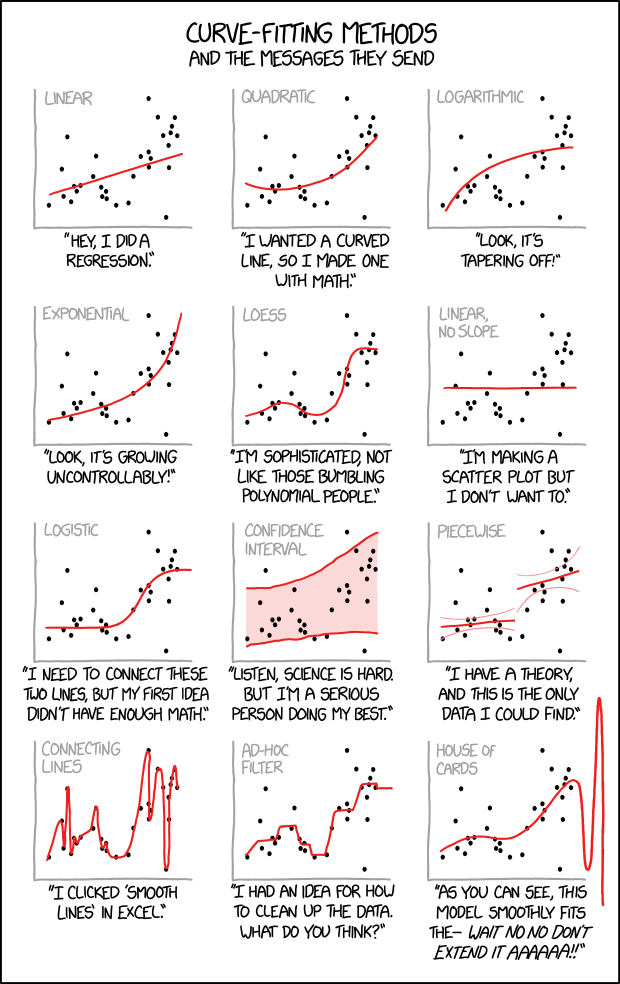
\includegraphics[height=0.55\textheight]{images/2048_curve_fitting.png}
\end{center}
\bottomnote{XKCD \#2048 by Randall Munroe (CC BY-NC 2.5)}
\end{frame}

% SLIDE 3: Learning Objectives
\begin{frame}[t]{Learning Objectives}
\vspace{1em}
After this lecture, you will be able to:
\begin{itemize}
  \item \textbf{Interpret} PCA and t-SNE visualizations to assess dimensionality reduction quality
  \item \textbf{Select} the optimal number of components using variance-based diagnostics
  \item \textbf{Compare} linear vs non-linear methods for different data structures
\end{itemize}
\bottomnote{We cover 20 essential visualizations spanning PCA foundations, t-SNE mechanics, and advanced topics}
\end{frame}

% SLIDE 4: Table of Contents
\begin{frame}{Outline}
  \tableofcontents
\bottomnote{Three parts: PCA Foundations, t-SNE and Non-Linear Methods, Comparison and Advanced Topics}
\end{frame}

% ============================================================
% PART 1: PCA FOUNDATIONS (7 charts)
% ============================================================
\section{PCA Foundations}

% SLIDE 5: C1 --- Scree Plot (REUSE)
\begin{frame}[t]{How Much Variance Does Each Component Capture?}
\begin{center}

\includegraphics[width=0.65\textwidth]{01_scree_plot/chart.pdf}
\end{center}
\bottomnote{The scree plot shows eigenvalues in descending order---look for the ``elbow'' where adding components yields diminishing returns}
\end{frame}

% SLIDE 6: C9 --- Cumulative Variance (NEW)
\begin{frame}[t]{How Many Components Do We Need?}
\begin{center}

\includegraphics[width=0.65\textwidth]{top10_09_cumulative_variance/chart.pdf}
\end{center}
\bottomnote{The cumulative variance curve answers the key question: how many PCs are needed for 90\% or 95\% of total variance?}
\end{frame}

% SLIDE 7: C2 --- PCA 2D Projection (REUSE)
\begin{frame}[t]{Projecting Data onto Principal Components}
\begin{center}

\includegraphics[width=0.60\textwidth]{02_principal_components/chart.pdf}
\end{center}
\bottomnote{PCA finds orthogonal directions of maximum variance and projects data onto them}
\end{frame}

% SLIDE 8: C10 --- Biplot (NEW)
\begin{frame}[t]{PCA Biplot: Which Features Drive Each Component?}
\begin{center}

\includegraphics[width=0.65\textwidth]{top10_10_pca_biplot/chart.pdf}
\end{center}
\bottomnote{Biplots overlay data scores with feature loading arrows---arrow direction shows which features align with each PC}
\end{frame}

% SLIDE 9: A4 --- Loading Heatmap (NEW)
\begin{frame}[t]{Feature Contributions Across Components}
\begin{center}

\includegraphics[width=0.65\textwidth]{top10_14_explained_var_heatmap/chart.pdf}
\end{center}
\bottomnote{Loading heatmaps reveal which features contribute most (positive or negative) to each principal component}
\end{frame}

% SLIDE 10: C3 --- Reconstruction (REUSE)
\begin{frame}[t]{Information Loss at Different Dimensions}
\begin{center}

\includegraphics[width=0.65\textwidth]{03_reconstruction/chart.pdf}
\end{center}
\bottomnote{Reconstruction error quantifies how much information is lost when projecting to fewer dimensions}
\end{frame}

% SLIDE 11: A1 --- Scaling Effect (NEW)
\begin{frame}[t]{Why Feature Scaling Is Non-Negotiable for PCA}
\begin{center}

\includegraphics[width=0.65\textwidth]{top10_11_scaling_effect/chart.pdf}
\end{center}
\bottomnote{Without scaling, PCA is dominated by high-variance features regardless of their informative content}
\end{frame}

% ============================================================
% TRANSITION
% ============================================================

% SLIDE 12: Transition
\begin{frame}[t]{From Linear to Non-Linear}
\vspace{1.5em}
\begin{itemize}
  \item PCA captures \highlight{global linear structure} but fails on curved manifolds
  \item t-SNE preserves \highlight{local neighbourhood structure} in low dimensions
  \item Kernel PCA extends PCA to non-linear settings via the kernel trick
\end{itemize}
\bottomnote{When data lies on a non-linear manifold, linear projections distort the true structure}
\end{frame}

% ============================================================
% PART 2: t-SNE AND NON-LINEAR METHODS (6 charts)
% ============================================================
\section{t-SNE and Non-Linear Methods}

% SLIDE 13: C4 --- t-SNE Perplexity=30 (REUSE)
\begin{frame}[t]{t-SNE: Preserving Local Structure}
\begin{center}

\includegraphics[width=0.65\textwidth]{04b_tsne_perplexity_30/chart.pdf}
\end{center}
\bottomnote{t-SNE converts pairwise similarities to probabilities and minimizes KL divergence between high- and low-dimensional distributions}
\end{frame}

% SLIDE 14: A10 --- Perplexity Grid (NEW)
\begin{frame}[t]{Effect of Perplexity on t-SNE}
\begin{center}

\includegraphics[width=0.65\textwidth]{top10_20_tsne_perplexity_grid/chart.pdf}
\end{center}
\bottomnote{Perplexity controls the effective number of neighbours---low values emphasise local, high values emphasise global structure}
\end{frame}

% SLIDE 15: A3 --- t-SNE Iterations (NEW)
\begin{frame}[t]{t-SNE Convergence Over Iterations}
\begin{center}

\includegraphics[width=0.65\textwidth]{top10_13_tsne_iterations/chart.pdf}
\end{center}
\bottomnote{Too few iterations produce noisy embeddings; convergence typically requires 500--1000 iterations}
\end{frame}

% SLIDE 16: C5 --- Swiss Roll PCA (REUSE)
\begin{frame}[t]{When PCA Fails: The Swiss Roll}
\begin{center}

\includegraphics[width=0.65\textwidth]{05a_pca_swiss_roll/chart.pdf}
\end{center}
\bottomnote{PCA projects the Swiss Roll onto a plane, collapsing the manifold structure and mixing distant points}
\end{frame}

% SLIDE 17: C6 --- Swiss Roll t-SNE (REUSE)
\begin{frame}[t]{When t-SNE Succeeds: Unrolling the Manifold}
\begin{center}

\includegraphics[width=0.65\textwidth]{05b_tsne_swiss_roll/chart.pdf}
\end{center}
\bottomnote{t-SNE preserves local distances along the manifold, successfully ``unrolling'' the Swiss Roll}
\end{frame}

% SLIDE 18: A2 --- Kernel PCA (NEW)
\begin{frame}[t]{Kernel PCA: Linear Methods on Non-Linear Data}
\begin{center}

\includegraphics[width=0.65\textwidth]{top10_12_kernel_pca/chart.pdf}
\end{center}
\bottomnote{Kernel PCA maps data to a higher-dimensional space where linear separation becomes possible}
\end{frame}

% ============================================================
% PART 3: COMPARISON AND ADVANCED TOPICS (7 charts)
% ============================================================
\section{Comparison and Advanced Topics}

% SLIDE 19: C7 --- PCA Clusters (REUSE)
\begin{frame}[t]{PCA Cluster Projection}
\begin{center}

\includegraphics[width=0.65\textwidth]{06b_pca_cluster_projection/chart.pdf}
\end{center}
\bottomnote{PCA preserves global variance but may overlap clusters that are separated in higher dimensions}
\end{frame}

% SLIDE 20: C8 --- t-SNE Clusters (REUSE)
\begin{frame}[t]{t-SNE Cluster Projection}
\begin{center}

\includegraphics[width=0.65\textwidth]{06c_tsne_cluster_projection/chart.pdf}
\end{center}
\bottomnote{t-SNE excels at separating clusters by preserving local neighbourhood relationships}
\end{frame}

% SLIDE 21: A6 --- Distance Preservation (NEW)
\begin{frame}[t]{Does t-SNE Preserve Distances?}
\begin{center}

\includegraphics[width=0.65\textwidth]{top10_16_tsne_distance_preservation/chart.pdf}
\end{center}
\bottomnote{t-SNE preserves local distances well but distorts global distances---inter-cluster gaps are not meaningful}
\end{frame}

% SLIDE 22: A7 --- Runtime (NEW)
\begin{frame}[t]{PCA vs t-SNE: Runtime Comparison}
\begin{center}

\includegraphics[width=0.65\textwidth]{top10_17_pca_vs_tsne_runtime/chart.pdf}
\end{center}
\bottomnote{PCA scales linearly; t-SNE scales quadratically. For large datasets, run PCA first to reduce dimensions before t-SNE}
\end{frame}

% SLIDE 23: A5 --- Denoising (NEW)
\begin{frame}[t]{PCA for Denoising: Recovering Signal from Noise}
\begin{center}

\includegraphics[width=0.65\textwidth]{top10_15_pca_denoising/chart.pdf}
\end{center}
\bottomnote{Projecting onto top PCs and reconstructing removes noise captured by lower components}
\end{frame}

% SLIDE 24: A9 --- Whitening (NEW)
\begin{frame}[t]{PCA Whitening: Decorrelation and Scaling}
\begin{center}

\includegraphics[width=0.65\textwidth]{top10_19_pca_whitening/chart.pdf}
\end{center}
\bottomnote{Whitening decorrelates features and scales them to unit variance---often used as preprocessing for neural networks}
\end{frame}

% SLIDE 25: A8 --- Intrinsic Dim (NEW)
\begin{frame}[t]{Finding the Intrinsic Dimensionality}
\begin{center}

\includegraphics[width=0.65\textwidth]{top10_18_intrinsic_dimensionality/chart.pdf}
\end{center}
\bottomnote{The elbow in explained variance reveals the true number of informative dimensions in the data}
\end{frame}

% ============================================================
% CLOSING
% ============================================================
\section{Summary}

% SLIDE 26: Summary Checklist
\begin{frame}[t]{20 Charts You Should Know}
\vspace{0.3em}
\begin{columns}[T]
\begin{column}{0.48\textwidth}
\footnotesize
\begin{enumerate}
  \item[\checkmark] Scree Plot
  \item[\checkmark] Cumulative Variance
  \item[\checkmark] 2D Projection
  \item[\checkmark] Biplot
  \item[\checkmark] Loading Heatmap
  \item[\checkmark] Reconstruction
  \item[\checkmark] Scaling Effect
  \item[\checkmark] Kernel PCA
  \item[\checkmark] t-SNE Iterations
  \item[\checkmark] Perplexity Grid
\end{enumerate}
\end{column}
\begin{column}{0.48\textwidth}
\footnotesize
\begin{enumerate}
  \item[\checkmark] t-SNE Perplexity
  \item[\checkmark] Swiss Roll (PCA)
  \item[\checkmark] Swiss Roll (t-SNE)
  \item[\checkmark] PCA Clusters
  \item[\checkmark] t-SNE Clusters
  \item[\checkmark] Distance Preservation
  \item[\checkmark] Runtime
  \item[\checkmark] Denoising
  \item[\checkmark] Whitening
  \item[\checkmark] Intrinsic Dimensionality
\end{enumerate}
\end{column}
\end{columns}
\bottomnote{These 20 visualizations cover the foundations, mechanics, and interpretation of dimensionality reduction}
\end{frame}

% SLIDE 27: Closing XKCD
\begin{frame}[t]{The Signal in the Noise}
\vspace{0.5em}
\begin{center}

\includegraphics[height=0.55\textheight]{images/2400_statistics.png}
\end{center}
\bottomnote{XKCD \#2400 by Randall Munroe (CC BY-NC 2.5)}
\end{frame}

\end{document}
